%%%%%%%%%%%%%%%%%%%%%%%%%%%%%%%%%%%%%%%%%
% Diaz Essay
% LaTeX Template
% Version 2.0 (13/1/19)
%
% This template originates from:
% http://www.LaTeXTemplates.com
%
% Authors:
% Vel (vel@LaTeXTemplates.com)
% Nicolas Diaz (nsdiaz@uc.cl)
%
% License:
% CC BY-NC-SA 3.0 (http://creativecommons.org/licenses/by-nc-sa/3.0/)
%
%%%%%%%%%%%%%%%%%%%%%%%%%%%%%%%%%%%%%%%%%

%----------------------------------------------------------------------------------------
%	PACKAGES AND OTHER DOCUMENT CONFIGURATIONS
%----------------------------------------------------------------------------------------

\documentclass[11pt]{diazessay} % Font size (can be 10pt, 11pt or 12pt)
\usepackage{listings}

%----------------------------------------------------------------------------------------
%	TITLE SECTION
%----------------------------------------------------------------------------------------

\title{\textbf{NBA Data WareHouse}} % Title and subtitle

\author{\textbf{Bases de Datos Avanzadas} \\ \textit{Escuela Superior Informática (UCLM)}} % Author and institution

\date{\today} % Date, use \date{} for no date

%----------------------------------------------------------------------------------------

\begin{document}

\maketitle % Print the title section

%----------------------------------------------------------------------------------------
%	ABSTRACT AND KEYWORDS
%----------------------------------------------------------------------------------------

%\renewcommand{\abstractname}{Summary} % Uncomment to change the name of the abstract to something else

\begin{abstract}

\end{abstract}

%\hspace*{3.6mm}\textit{Keywords:} lorem, ipsum, dolor, sit amet, lectus % Keywords

\vspace{30pt} % Vertical whitespace between the abstract and first section

%----------------------------------------------------------------------------------------
%	ESSAY BODY
%----------------------------------------------------------------------------------------

\section*{Introducción}
Un almacén de datos o \textit{Data Warehouse} es el instrumento que las organizaciones encontraron centralizar toda la información relevante, el objetivo de tomar decisiones informadas con más facilidad. Es decir, facilitar el almacenaje y análisis de los datos de la empresa.\\

En nuestro caso, hemos construido un almacén de datos para almacenar las estadísticas mas relevantes de la temporada 2018-2019 de la competición de baloncesto más popular, la NBA \cite{nba}. El trabajo consiste en la extracción de datos de la competición disponibles en \cite{basket_ref} y almacenaje de estos datos en una base datos relacional para su posterior estudio.\\

Para el análisis y la extracción de datos, se llevará a cabo el proyecto con \textit{Python} \cite{python} y como motor de base de datos se utilizará \textit{SQLite} \cite{sqlite}. Nuestra base de datos estará formada por cuatro tablas, que se describirán posteriormente.

%------------------------------------------------
\clearpage

\section*{Obtención de los datos}
Los datos se han obtenido aplicando técnicas de \textit{web scraping} \cite{web_scraping} gracias a la librería \textit{Beautiful Soup} \cite{Beautiful_Soup} de \textit{Python}. Con esta librería se obtiene el código HTML de una pagina web y se pueden realizar diversas operaciones con esa información, en nuestro caso hemos construido un \textit{dataframe} \cite{dataframe} para poder construir posteriormente la base de datos.

\subsection*{Datos de jugadores}
Los datos relacionados con los jugadores se han obtenido gracias al siguiente código \cite{web_scraping_nba} en \textit{Python}:\\

\pythonexternal{../player_stats.py}

Como se puede ver, el programa esta formado por dos funciones. La primera para obtener las estadísticas globales de todos los jugadores \cite{players_data} y con la segundo se obtienen los datos relativos a los \textit{rookies} (jugadores nóveles) \cite{rookies_data}. Ambas funciones devolverán un objeto \textit{dataframe} \cite{dataframe}, porque en el programa principal se llamará a estas funciones para construir la base de datos, como se ha comentado anteriormente. Para el tratamiento de los datos en forma de \textit{dataframe} utilizaremos la librería \textit{pandas} \cite{pandas}.\\

Para obtener los datos que nos interesan de la web es necesario que sepamos cuáles son las etiquetas HTML que debemos de obtener del objeto \textit{soup}. Esto normalmente se realiza inspeccionando la página web con cualquier navegador.

\subsection*{Datos de equipos}
Los datos relativos a los equipos de la \textit{nba} se han obtenido de forma similar a los datos de los jugadores:

\pythonexternal{../team_stats.py}

La función para obtener los datos de los equipos es muy similar a las funciones mencionadas anteriormente, con la diferencia que el \textit{dataframe} que retornamos lo ordenamos por el nombre del equipo. La segunda función en un principio no la desarrollamos, pero en la construcción de la base de datos apreciamos que los datos de los jugadores indican el equipo mediante abreviaturas. Por lo tanto esta función la utilizaremos para establecer las equivalencias.

\clearpage

\section*{Creación de la base de datos}
La creación de la base de datos la hemos automatizado gracias al siguiente \textit{script} que llama a las funciones explicadas en la sección anterior:

\pythonexternal{../build_database.py}

El programa lleva a cabo las siguientes operaciones:
\begin{itemize}
	\item \textbf{Cargar los datos:} se llama a las funciones explicadas anteriormente para cargar la información relativas a jugadores, \textit{rookies} y equipos.  Además, en esta parte del programa también se establece la equivalencia de los equipos con sus abreviaturas.
	\item \textbf{Transformación de datos:} se realiza una limpieza de los datos, que consiste en eliminar las columnas que no vamos a utilizar, eliminar las filas vacías y eliminación de jugadores que no juegan en un equipo de la nba.
	\item \textbf{Construcción del \textit{dataframe} central}: estos datos se usarán para construir una tabla central que relacione los datos de jugadores, \textit{rookies} y equipos, siguiendo el modelo de estrella \cite{estrella}.
	\item \textbf{Construcción de la base datos}: en este último paso se construirán las cuatro tablas de la base datos y se introducirán los datos guardados en los cuatro \textit{dataframes} que hemos comentado. Las operaciones que se ejecutan para crear las tabla y sus respectivas relaciones se pueden ver en el fichero \textit{\textbf{creation.sql}}.
\end{itemize}

\subsection*{Diagrama relacional}
El diagrama relacional de nuestra base de datos, estará formado por cuatro tablas relacionadas en forma de estrella, de las cuales tres de ellas las crearemos a partir de los datos obtenidos en el punto anterior (\textit{Equipos}, \textit{Jugadores} y \textit{Rookies}). La cuarta tabla (\textit{Jugadores-Equipos}) es una tabla central, la cual está relacionada con cada una de las anteriores tablas.

\begin{figure}[h!]
	\centering
	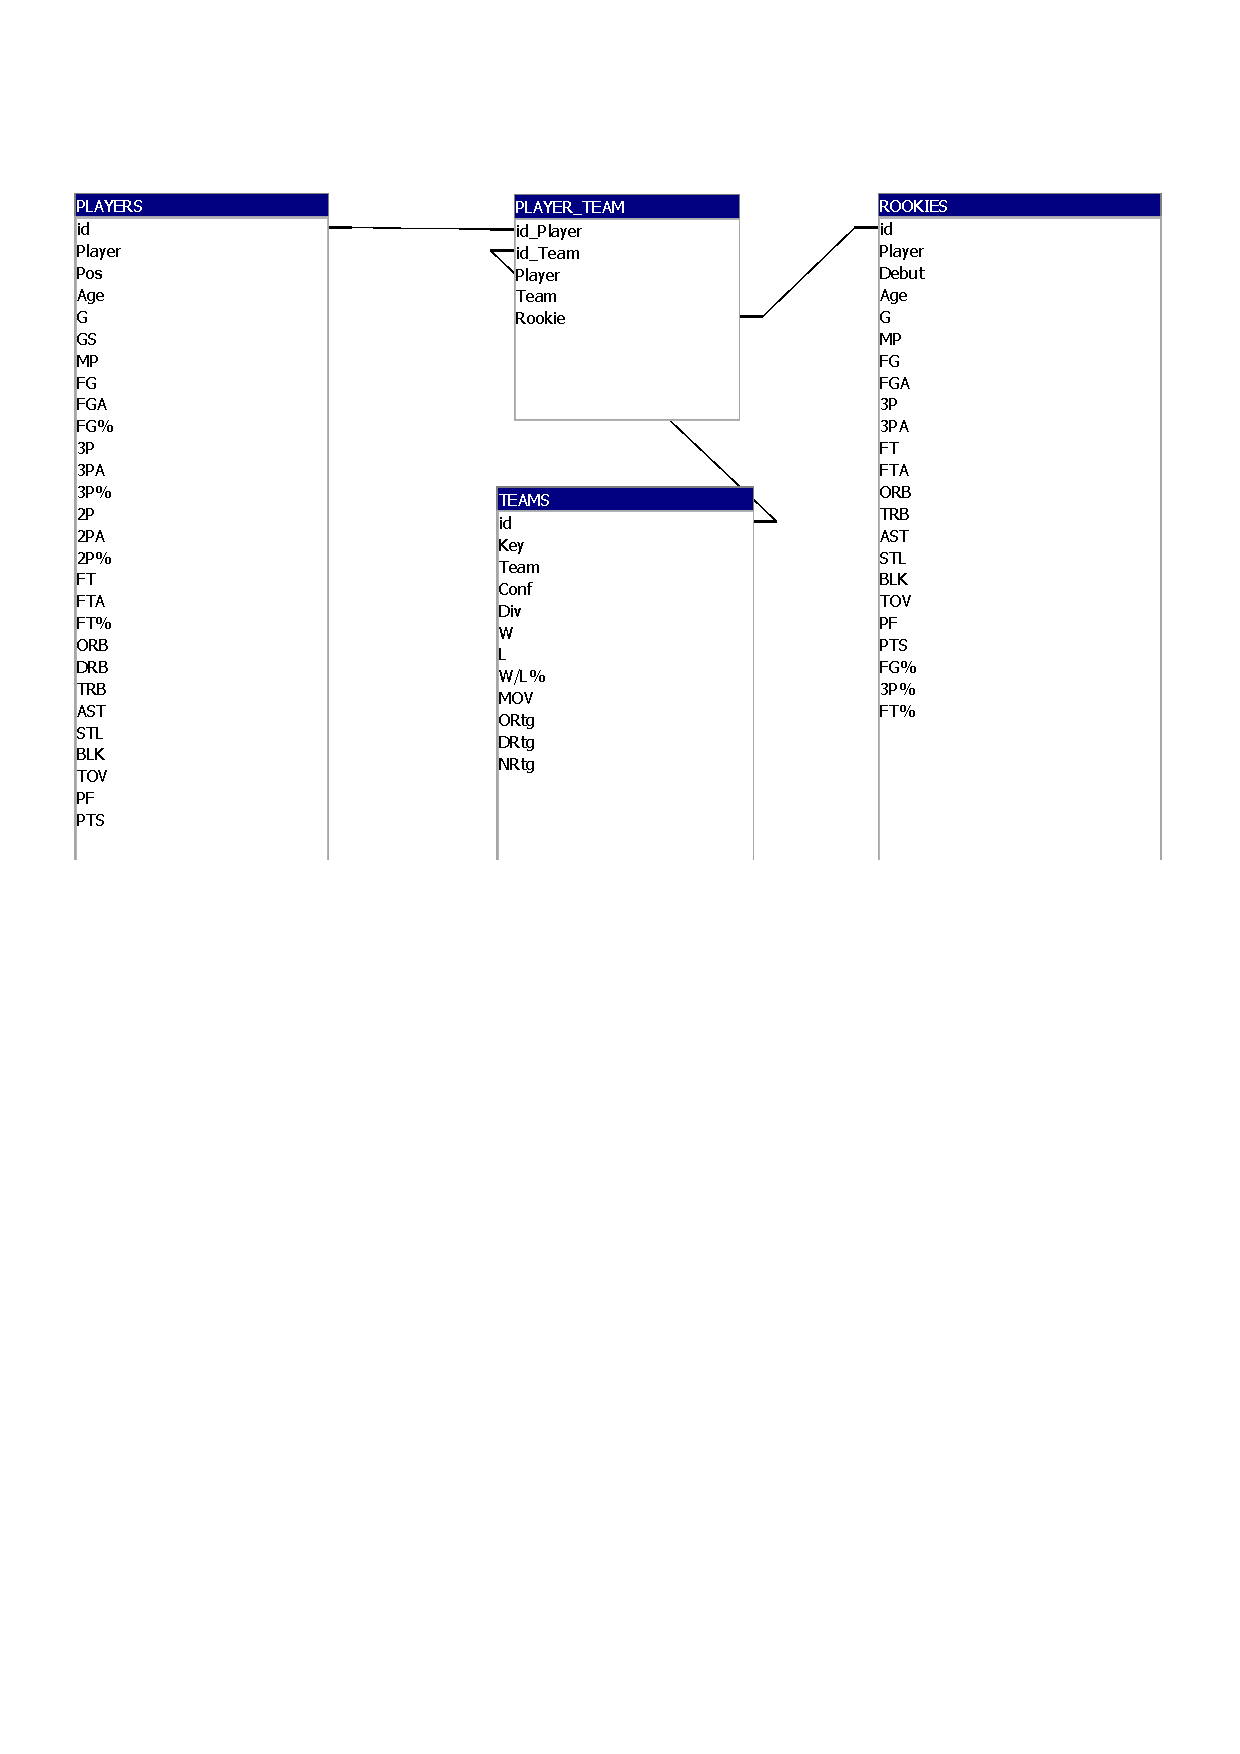
\includegraphics[width=1\linewidth]{bd_dRelacional.pdf}
	\caption{Diagrama relacional de nuestra base de datos}
	\label{fig:diagrama}
\end{figure}

A continuación, se explicara la definición de cada parametro por los que está formada cada tabla.\\

La tabla \textbf{Jugadores} (PLayers), esta formada por:
\begin{itemize}
	\item \textbf{id}: Player id.
	\item \textbf{Player}: Player full name.
	\item \textbf{Pos}: Position.
	\item \textbf{Age}: Player age.
	\item \textbf{G}: Games.
	\item \textbf{GS}: Games started
	\item \textbf{MP}: Minutes played.
	\item \textbf{FG (3P + 2P)}: Field goals.
	\item \textbf{FGA (3PA + 2PA)}: Field goal attempts.
	\item \textbf{FG\%}: Field goal percentage.
	\item \textbf{3P}: 3 points field goals.
	\item \textbf{3PA}: 3 point field goal attempts.
	\item \textbf{3P\%}: FG\% on 3 points FGA's (field goal attempts).
	\item \textbf{2P}: 2 points field goals.	
	\item \textbf{2PA}: 2 point field goal attempts.
	\item \textbf{2P\%}: FG\% on 2 points FGA's (field goal attempts).
	\item \textbf{FT}:Free Throwns.
	\item \textbf{FTA}:Free Thrown Attempts.
	\item \textbf{FT\%}: Free Throw Percentage.
	\item\textbf{ORB}: Offensive Rebounds.
	\item\textbf{DRB}: Defensive Rebounds.
	\item\textbf{TRB}: Total Rebounds
	\item\textbf{AST}: Assists.
	\item\textbf{STL}: Steals.
	\item\textbf{BLK}: Blocks.
	\item\textbf{TOV}:Turnovers.
	\item\textbf{PF}: Personal Fouls.
	\item\textbf{PTS}: Points.
\end{itemize}

La tabla \textbf{Equipos} (Teams), esta formada por:
\begin{itemize}
	\item \textbf{id}: Team id.
	\item \textbf{Key}: Team initials.
	\item \textbf{Team}: Team name.
	\item \textbf{Conf}: Team's conference.
	\item \textbf{Div}: Team's division.
	\item \textbf{W}: Wins.
	\item \textbf{L}: Losses.
	\item \textbf{W/L\%}: Win-Loss Percentage.
	\item \textbf{MOV}: Margin of Victory.
	\item\textbf{ORTg}: Offensive Rating. An estimate of points produced (\textit{players}) or scored (\textit{teams}) per 100 possessions.
	\item\textbf{DRTg}: Defensive Rating. An estimate of points allowed per 100 possessions.
	\item\textbf{NRTg}: Net Rating. An estimate of point differential per 100 possessions.
\end{itemize}

La tabla \textbf{Rookies}, esta formada por:
\begin{itemize}
	\item \textbf{id}: Rookie id.
	\item \textbf{Player}: Player full name.
	\item \textbf{Debut}: Debut.
	\item \textbf{Age}: Player age.
	\item \textbf{G}: Games.
	\item \textbf{MP}: Minutes played.
	\item \textbf{FG (3P + 2P)}: Field goals.
	\item \textbf{FGA (3PA + 2PA)}: Field goal attempts.
	\item \textbf{3P}: 3 points field goals.
	\item \textbf{3PA}: 3 point field goal attempts.
	\item \textbf{3P\%}: FG\% on 3 points FGA's (field goal attempts).
	\item \textbf{FT}:Free Throwns.
	\item \textbf{FTA}:Free Thrown Attempts.
	\item \textbf{FT\%}: Free Throw Percentage.
	\item\textbf{ORB}: Offensive Rebounds.
	\item\textbf{DRB}: Defensive Rebounds.
	\item\textbf{TRB}: Total Rebounds
	\item\textbf{AST}: Assists.
	\item\textbf{STL}: Steals.
	\item\textbf{BLK}: Blocks.
	\item\textbf{TOV}:Turnovers.
	\item\textbf{PF}: Personal Fouls.
	\item\textbf{PTS}: Points.
\end{itemize}

La tabla \textbf{Jugadores-Equipos} (Players-Teams), esta formada por:
\begin{itemize}
	\item\textbf{id-Player}: Player id.
	\item\textbf{id-Team}: Team id.
	\item\textbf{Player}: Player full name.
	\item\textbf{Team}: Team name.
	\item\textbf{Rookie}: Rookie id. If \textit{player} is a \textit{rookie}, then \textit{id-Rookie} stores in this attribute.
\end{itemize}

\clearpage

\section{Obtención de estadísticas}
A continuación, se realizarán una serie de consultas para obtener información sobre algunas estadísticas sobre los jugadores y los equipos de esta temporada. Para ver la gran utilidad que puede aportar la unión de estas dos tecnologías \textit{SQLite} y \textit{Python}.\\

Para facilitar la obtención de los datos se han generado una serie de \textit{vistas SQL}, las cuales están almacenadas en nuestra base de datos (\textit{nba-data.db}). \\

Estas son las siguientes:
\pythonexternal{../Queries.sql}


\subsection{Porcentaje de jugadores y rookies de la temporada.}
Mediante un diagrama en forma de "pastel" se puede observar de forma rápida e intutiva en este caso, los jugadores \textit{rookies} y no \textit{rookies} que jugaron esta temporada.

Lo mas importante es generar bien la consulta, a partir de la cual se va a generar el \textit{dataframe}:\\

\textit{"SELECT * FROM STAT-PT"}

\begin{figure}[!h]
	\centering
	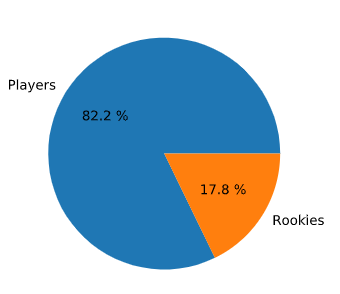
\includegraphics[width=0.5\linewidth]{rookies.png}
	\caption{Porcentaje de jugadores y rookies de la temporada.}
	\label{fig:rookies}
\end{figure}

\subsection{Número de jugadores y rookies de cada conferencia}
Se obtendrán los datos sobre el numero de jugadores y número de rookies de cada conferencia. 

Para poder obtener los datos se ha utlizado la siguiente consulta \textit{SQL}:\\

\textit{"SELECT Conference, SUM(NoRookies-Perc) AS "PlayersPerc",SUM(RookiesPerc) AS "RookiesPerc" FROM STAT-PT GROUP BY Conference;"}

\begin{figure}[!h]
	\centering
	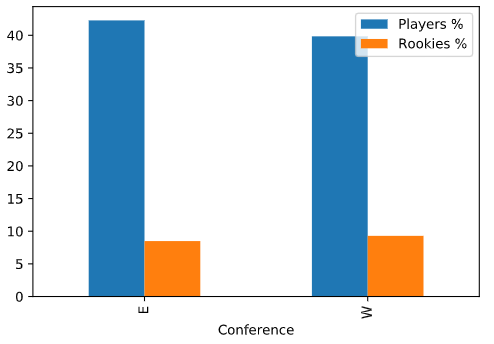
\includegraphics[width=0.5\linewidth]{rookies-conf.png}
	\caption{Porcentaje de jugadores y rookies por conferencia.}
	\label{fig:rookies-conf}
\end{figure}

\subsection{Número de jugadores que tiene cada equipo}
Se obtendra el número de jugadores que componen cada equipo de la temporada, los datos han sido obtenidos a partir de la siguiente consulta:\\

\textit{"SELECT * FROM NUM-PT"}

\begin{figure}[!h]
	\centering
	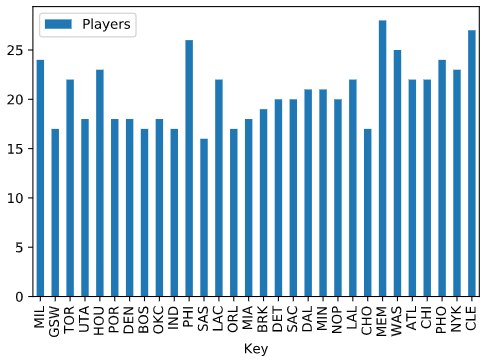
\includegraphics[width=0.5\linewidth]{teams.png}
	\caption{Número de jugadores que tiene cada equipo.}
	\label{fig:teams}
\end{figure}

\subsection{Simulación clasificación final de la temporada}
Se mostrará la clasificación final de la temporada. Sin tener en cuenta la conferencia a la que pertenece cada equipo, ni los \textit{playoffs}. 
Se han obtenidos los datos de la base de datos a partir de la siguiente consulta:\\

\textit{"SELECT Key, Team, Conf, W, L FROM TEAMS ORDER BY W/L DESC;"}

\begin{table}[!h]
	\centering
	\begin{tabular}{|c|c|l|c|}
		\hline
		\textbf{Pos} & \textbf{Key} & \multicolumn{1}{c|}{\textbf{Team}} & \textbf{Conf} \\ \hline
		\textbf{1}   & MIL          & Milwaukee Bucks                    & E             \\ \hline
		\textbf{2}   & TOR          & Toronto Raptors                    & E             \\ \hline
		\textbf{3}   & GSW          & Golden State Warriors              & W             \\ \hline
		\textbf{4}   & DEN          & Denver Nuggets                     & W             \\ \hline
		\textbf{5}   & HOU          & Houston Rockets                    & W             \\ \hline
		\textbf{6}   & POR          & Portland Trail Blazers             & W             \\ \hline
		\textbf{7}   & PHI          & Philadelphia 76ers                 & E             \\ \hline
		\textbf{8}   & UTA          & Utah Jazz                          & W             \\ \hline
		\textbf{9}   & BOS          & Boston Celtics                     & E             \\ \hline
		\textbf{10}  & OKC          & Oklahoma City Thunder              & W             \\ \hline
	\end{tabular}
	\caption{Clasificación final de la temporada (sin \textit{Playoffs}).}
	\label{qualy}
\end{table}

\subsection{Obtener la información del mejor equipo de cada conferencia.}
Se obtendrá la información del mejor equipo de cada conferencia, en este caso : Este (E): \textit{Milwaukee Bucks}, Oeste (W):
\textit{Golden State Warriors}. 
Se ha utilizado la siguiente consulta:\\
 
\textit{"SELECT * FROM TEAMS GROUP BY CONF HAVING MAX(W/L);"}

\begin{table}[!h]
	\centering
	\begin{tabular}{|l|l|l|l|l|l|l|l|l|l|}
		\hline
		\textbf{Key} & \textbf{Team}         & \textbf{Conf} & \textbf{W} & \textbf{L} & \textbf{W/L \%} & \textbf{MOV} & \textbf{ORtg} & \textbf{DRtg} & \textbf{NRtg} \\ \hline
		MIL          & Milwaukee Bucks       & E             & 60         & 22         & 0.732           & 8.87         & 114.23        & 105.76        & 8.47          \\ \hline
		GSW          & Golden State Warriors & W             & 57         & 25         & 0.695           & 6.46         & 116.63        & 110.24        & 6.39          \\ \hline
	\end{tabular}
	\caption{Primer equipo de cada conferencia (E/W)}
	\label{teamConf}
\end{table}

\clearpage

\section*{Modelo de regresión lineal}
El modelo construido está basado en la regresión lineal simple de dos variables \cite{regresion}, los puntos totales que anota un jugador con sus intentos de tiro. El objetivo con este modelo será predecir cuántos puntos anotaría un jugador indicando los intentos de tiro.\\

Los modelos predictivos o de regresión consisten en la representación de la relación entre dos (o más) variables a través de un modelo formal supone contar con una expresión lógico-matemática que resume cómo es esa relación. Además, este modelo permite realizar predicciones de los valores que tomará una de las dos variables (la que se asuma como variable de respuesta o dependiente, \textit{y}) a partir de los valores de la otra (la que se asuma como variable explicativa, independiente o predictora, \textit{x}) \cite{modelo_regresion}.\\

\subsection*{Cálculo del modelo}

En nuestro caso, como vamos a realizar una regresión lineal simple la formula sería la siguiente:\\

\begin{equation}
\centering
y = \alpha + \beta * x
\end{equation}
\\
La variable que queremos predecir (\textit{y}) serán los puntos que anotará un jugador y para ello utilizaremos la variable explicativa de los tiros a canasta de un jugador (x), contando los tiros libres, los tiros de dos puntos y los triples. \\

\begin{equation}
\centering
PTS = \alpha + \beta * TA
\end{equation}
\\
Los parámetros utilizados en la predicción se van a calcular utilizando la librería \textit{statsmodels} \cite{statsmodels} de Python. Los pasos seguidos para calcular este modelo se pueden ver con detalle en el \textit{notebook} de \textit{Jupyter} \cite{jupyter} que hemos creado. La fórmula resultante con los parámetros calculados en base a los datos almacenados en nuestro \textit{data warehouse} es la siguiente:\\
\begin{equation}
\centering
PTS = -5.209429 + 1.000137 * TA
\end{equation}
\\
Al dibujar la recta de regresión \cite{recta} podemos observar como de bueno es el modelo creado para predecir los puntos que anotará un jugador introduciendo los intentos a canasta (ver Figura \ref{fig:recta}). Cuanto menos dispersos y más cercanos a la recta estén los puntos mejor será nuestro modelo.

\begin{figure}[!h]
	\centering
	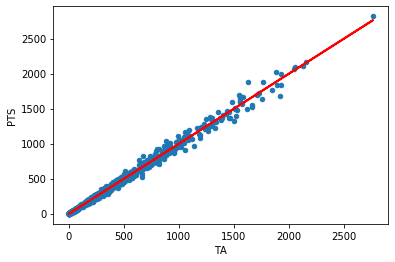
\includegraphics[width=0.8\linewidth]{recta_regresion.png}
	\caption{Recta de regresión de PTS~TA}
	\label{fig:recta}
\end{figure}

\subsection*{Realizar predicción}
En este punto, se va a realizar una serie de predicciones utilizando la expresión calculada anteriormente. En el Cuadro \ref{pred} se pueden ver cinco jugadores con los puntos reales anotados en la temporada y los puntos que predice nuestro modelo. Se puede apreciar que la predicción se asemeja bastante a los puntos que anota un jugador. \\

\begin{table}[!h]
	\centering
	\begin{tabular}{|l|l|l|}
		\hline
		\textbf{Player} & \textbf{PTS} & \textbf{PTS\_pred} \\ \hline
		Álex Abrines    & 165          & 164.813847         \\ \hline
		Quincy Acy      & 17.0         & 22.794404          \\ \hline
		Jaylen Adams    & 108.0        & 113.806864         \\ \hline
		Steven Adams    & 1108.0       & 1095.941316        \\ \hline
		Bam Adebayo     & 729.0        & 706.888055         \\ \hline
	\end{tabular}
	\caption{Predicciones del modelo}
	\label{pred}
\end{table}

Cabe destacar que los parámetros han sido calculados con los mismos datos que luego hemos usado para predecir, por lo tanto, se puede dar el fenómeno de la multicolinealidad \cite{multicol}. Esto sucede cuando el modelo se ajusta demasiado a un conjunto de datos y cuando utilizamos otros datos para hacer una predicción el modelo falla. \\

En nuestro caso, al usar datos de una temporada de una competición deportiva se presupone que los datos no van a ser muy desiguales de una temporada a otra. Con lo cual, nuestro modelo se debe comportar correctamente cuando introducimos un dato que no forma parte del conjunto utilizado para crear el modelo.

\newpage





%Cras gravida, est vel interdum euismod, tortor mi lobortis mi, quis adipiscing elit lacus ut orci. Phasellus nec fringilla nisi, ut vestibulum neque. Aenean non risus eu nunc accumsan condimentum at sed ipsum.
%\begin{wrapfigure}{l}{0.42\textwidth} % Inline image example, use an 'r' column type to position the figure on the right
%	
\includegraphics[width=\linewidth]{fish.png}
%	\caption{An example fish.}
%\end{wrapfigure}
%Aliquam fringilla non diam sed varius. Suspendisse tellus felis, hendrerit non bibendum ut, adipiscing vitae diam. Lorem ipsum dolor sit amet, consectetur adipiscing elit. Nulla lobortis purus eget nisl scelerisque, commodo rhoncus lacus porta. Vestibulum vitae turpis tincidunt, varius dolor in, dictum lectus. Aenean ac ornare augue, ac facilisis purus. Sed leo lorem, molestie sit amet fermentum id, suscipit ut sem. Vestibulum orci arcu, vehicula sed tortor id, ornare dapibus lorem. Praesent aliquet iaculis lacus nec fermentum. Morbi eleifend blandit dolor, pharetra hendrerit neque ornare vel. Nulla ornare, nisl eget imperdiet ornare, libero enim interdum mi, ut lobortis quam velit bibendum nibh.
%
%\begin{itemize}
%	\item First bullet point item
%	\item Second bullet point item
%	\item Third bullet point item
%\end{itemize}
%
%Morbi tempor congue porta. Proin semper, leo vitae faucibus dictum, metus mauris lacinia lorem, ac congue leo felis eu turpis. Sed nec nunc pellentesque, gravida eros at, porttitor ipsum. Praesent consequat urna a lacus lobortis ultrices eget ac metus. In tempus hendrerit rhoncus. Mauris dignissim turpis id sollicitudin lacinia. Praesent libero tellus, fringilla nec ullamcorper at, ultrices id nulla. Phasellus placerat a tellus a malesuada.
%
%\begin{enumerate}
%	\item First numbered list item
%	\item Second numbered list item
%\end{enumerate}

%------------------------------------------------

%\section*{Conclusion}
%
%Fusce in nibh augue. Cum sociis natoque penatibus et magnis dis parturient montes, nascetur ridiculus mus. In dictum accumsan sapien, ut hendrerit nisi. Phasellus ut nulla mauris. Phasellus sagittis nec odio sed posuere. Vestibulum porttitor dolor quis suscipit bibendum. Mauris risus lectus, cursus vitae hendrerit posuere, congue ac est. Suspendisse commodo eu eros non cursus. Mauris ultrices venenatis dolor, sed aliquet odio tempor pellentesque. Duis ultricies, mauris id lobortis vulputate, tellus turpis eleifend elit, in gravida leo tortor ultricies est. Maecenas vitae ipsum at dui sodales condimentum a quis dui. Nam mi sapien, lobortis ac blandit eget, dignissim quis nunc.
%
%Donec luctus tincidunt mauris, non ultrices ligula aliquam id. Sed varius, magna a faucibus congue, arcu tellus pellentesque nisl, vel laoreet magna eros et magna. Vivamus lobortis elit eu dignissim ultrices. Fusce erat nulla, ornare at dolor quis, rhoncus venenatis velit. Donec sed elit mi. Sed semper tellus a convallis viverra. Maecenas mi lorem, placerat sit amet sem quis, adipiscing tincidunt turpis. Cras a urna et tellus dictum eleifend. Fusce dignissim lectus risus, in bibendum tortor lacinia interdum.
%
%\begin{table}[h] % [h] forces the table to be output where it is defined in the code (it suppresses floating)
%	\caption{Example table.}
%	\centering
%	\begin{tabular}{l l r}
%		\toprule
%		\multicolumn{2}{c}{Name} \\
%		\cmidrule(r){1-2}
%		First Name & Last Name & Grade \\
%		\midrule
%		John & Doe & $7.5$ \\
%		Richard & Miles & $5$ \\
%		\bottomrule
%	\end{tabular}
%\end{table}
%
%Fusce eleifend porttitor arcu, id accumsan elit pharetra eget. Mauris luctus velit sit amet est sodales rhoncus. Donec cursus suscipit justo, sed tristique ipsum fermentum nec. Ut tortor ex, ullamcorper varius congue in, efficitur a tellus. Vivamus ut rutrum nisi. Phasellus sit amet enim efficitur, aliquam nulla id, lacinia mauris. Quisque viverra libero ac magna maximus efficitur. Interdum et malesuada fames ac ante ipsum primis in faucibus. Vestibulum mollis eros in tellus fermentum, vitae tristique justo finibus. Sed quis vehicula nibh. Etiam nulla justo, pellentesque id sapien at, semper aliquam arcu. Integer at commodo arcu. Quisque dapibus ut lacus eget vulputate.

%----------------------------------------------------------------------------------------
%	BIBLIOGRAPHY
%----------------------------------------------------------------------------------------

\bibliographystyle{abbrv}

\bibliography{sample.bib}

%----------------------------------------------------------------------------------------

\end{document}
